\documentclass{llncs}

\usepackage[utf8]{inputenc}
\usepackage{url}
\usepackage{graphicx}
\graphicspath{{./images/}}

\title{Using human-machine hybrid workflow in crowdsourcing open geospatial data}

\author{Gianfranco Cecconi}
\institute{University of Southampton \email{gc1a13@soton.ac.uk}}

\date{December 2015}

\begin{document}


\maketitle

\section{Introduction}

\subsection{Crowdsourcing}

Crowdsourcing is {[}...{]}. More generally {[}BLAH BLAH SOCIAL MACHINES AS POSSIBLY ONE OF THE ONLY WAYS TO SOLVE PROBLEMS LIKE THIS + SOME EXCUSE TO CITE \cite{OReilly:2015uo}{]}

\subsection{Crowdsourcing Geographic Information}

Among the many successful applications of crowdsourcing is the collection and maintenance of geospatial data, or "Geographic Information" (GI), as it is commonly referred to in literature.

Although it is commonly recognised for GI to have a significant economic and social value \cite{Sui:2012uf}[THIS IS A REFERENCE TO AN ENTIRE BOOK, LIKELY UNSUITABLE], the effort National Mapping and Cadastre Agencies (NMCAs) put into producing and updating cartography has been in decline for several decades \cite{ESTES:1994vz}. In the U.S., for example, the Geological Survey no longer attempts to update its maps on a regular basis and the National Research Council promotes a vision in which {[}...{]} \cite{Committee:1993vp}.

{[}Somewhere in the literature someone said that the emergence of VGI was actually suggested by one of those authorities{]}

Crowdsourcing GI is then seen as the cost effective and good enough*** solution to this problem. The phenomenon of {\it Volunteered} Geographic Information (VGI) in particular was studied extensively since the term was coined \cite{Goodchild:2007vt}. Developing understanding of VGI was made possible by the success of services such as Wikimapia\footnote{\url{http://wikimapia.org/}.} or OpenStreetMap\footnote{\url{http://www.openstreetmap.org/}.}. The latter is likely the best known VGI-based mapping service available today.

\subsection{Open data}

Open data is data that anyone can access, use and share\footnote{\url{http://theodi.org/faq}.}. 

NMCAs, as governments and private organisations, are becoming more sensitive to the opportunities arising from publishing and re-using open data. In Great Britain, for example, since 2015 the local NMCA Ordnance Survey\footnote{\url{http://www.ordnancesurvey.co.uk/}.} has released in the open a substantial volume of data that was previously available to the public as commercial products only, e.g. "Open Names"\footnote{\url{https://www.ordnancesurvey.co.uk/business-and-government/products/os-open-names.html}.}, a place name index, and "Open Roads"\footnote{\url{https://www.ordnancesurvey.co.uk/business-and-government/products/os-open-roads.html}.}, the generalised geometry and network connectivity of the road network.

The availability of such high quality and authoritative sources becomes a substantial catalyser for the creation of new GI. There were geospatial data could only be created from scratch - as in the case of OpenStreetMap when it was started in the UK in 2007 - it is now possible to rather focus the effort of the crowd on complementing the GI that is already available.

\subsection{Challenges of crowdsourcing geospatial data}

Challenges remain in making the most out of the advantage described above, that is a prerogative of GI in those countries where geospatial open data is published. In general, it is useful and relevant to identify what characteristics of crowdsourcing systems assure better performance in those situation where pre-existing data is available for integration, whatever the data represents. 

In this paper we propose methods for improving the performance of such crowdsourcing systems, measured as a combination of speed of production and quality of output. We leverage three factors in particular that were the subject to our experiments: a) the crowd capability to choose their tasks, b) the motivation arising from visibility of collective effort and c) the dynamic allocation of monetary rewards.

{[}
Add
\begin{itemize}
	\item {[}rationale of why we thought this was relevant, some justification in literature review{]}
	\item {[}novelty of what we propose{]}
\end{itemize}
{]}

{(}...{)}

{[}Definition of address{]}

Many complementary and/or alternative strategies are possible and need to be used jointly to build OLAF. Among these is the opportunity to re-use published open datasets of addresses so to infer the existence of more addresses. 

E.g. it is intuitive that if some source refers to the existence of house numbers 3, 5 and 9 in some street, and all are associated to the same postcode, it is very likely that number 7 exists as well and is associated to the same postcode\footnote{House numbering and postcode association are heavily dependant of the conventions used in the country the problem is applied to. This paper always refers to the UK conventions.}. It is shown experimentally that the method is effective, as it can produce large volumes of addresses from available open data\footnote{This was tested against the single largest known source of addresses open data for England and Wales: Land Registry's "Price Paid Data". See \url{https://www.gov.uk/government/collections/price-paid-data}.}.

The experiments described in this paper implement the above strategy only, and  use crowdsourcing to validate sets of inferred addresses, as participants are asked to virtually survey the streets using pictures sourced from Google Street View.

It has to be noted that not all existing house numbers are visible by surveying a street. E.g. there are no obligations in the UK to affix a house number or house name sign. Moreover, some of the house numbers may be associated to dwellings that are not visible unless the property is accessed, beyond what Google Street View's photos can capture.

{(}...{)}

\section{Crowdsourcing addresses: our approach}

\subsection{Task model}

The following is a description of the approach that was used for crowdsourcing addresses, that is common to all experimental conditions that were tested.

\textbf{Requester.} The Requester desires to validate the existence of a series of house numbers (e.g. "3" or "7A") in a specified street. Those were previously inferred algorithmically from the observation of \textit{existing} house numbers, as sourced from published open datasets\footnote{See the GitHub repository at \url{https://github.com/Digital-Contraptions-Imaginarium/OLAF-yr2_reference_data} to learn about the reference open data we used, and the repository at \url{https://github.com/Digital-Contraptions-Imaginarium/OLAF-yr2_inference_data} for the inference algorithms.}. When the pictures in the survey tool are of insufficient quality to be read intelligibly (e.g. a house number could be "7A" but it is not clear) it is useful to the Requester to be informed of that. The Requester requires the help of human agents to carry out the tasks, that we will call Workers in the following.

\textbf{Task.} Each HIT (Human Intelligence Task) consists of verifying the existence in a given street of a given specific tuple of inferred house numbers {[}SOME MATHS SYMBOLS HERE{]} that is a subset of the whole set of inferred house numbers for that street {[}SOME MATHS SYMBOLS HERE{]}. 

\textbf{Strategy.} 
{[}TO BE WRITTEN, DEPENDS ON THE EXPERIMENT SCENARIOS DEFINITION.{]}

\textbf{Crowd $\rightarrow$ Worker.} Each Worker performs her task by declaring, for each house number in the given tuple and street, if a) it can be found by using the survey tool, b) it can't be found or c) it cannot be said with certainty (e.g. if some of the pictures are blurred and could correspond to the house number being searched). Multiple Workers are asked to validate the same tuple and the resulting data is chosen through majority voting.

\textbf{Reliability.} When collecting data to build a dataset that is intended to be published under an open licence, the option to assess its \textit{quality} by comparison with other sources is often not available, for many reason. An alternative source of the same data could simply not be available. Moreover, from an intellectual property perspective, the comparison could make the former "derivative work" of the latter, hence compromising the purpose{[}SOME REFERENCE OR FOOTNOTE TO PUT MORE MEAT AROUND THIS POINT{]}. 

What is possible, instead, is to estimate the \textit{reliability} of the crowdsourced data, independently of any actual knowledge of other sources and/or the ground truth. 

In OLAF's case, the approach described is considered equivalent to what is used for crowdsourcing the acquisition of labels for data items when the labelling is imperfect, that is extensively covered in literature, e.g. in \cite{sheng2008get} or \cite{Welinder:2010vkb}{[STILL HAVE TO READ THE LATTER{]}. 

The quality of the Workers' contribution could be measured by using gold standard tasks \cite{Oleson:2011tx}, e.g. asking them to validate sets of house numbers whose existence is already known. Because of the elementary complexity of the tasks, though, it was assumed that anything standing between the Worker and the actual required tasks would hinder their contribution in volume and quality and compromise furtherance.

Lacking an assessment of the individual Worker's reliability, the option of preferring the best individual Workers vs using multiple labellers becomes unavailable, hence the need to use majority voting. 

For simplicity, all Workers are considered equivalent from a reliability perspective, and the quality of their individual output assumed $ > 0.5 $, so that the \textit{uniform labeller quality} (see \cite{sheng2008get}) of the data chosen through majority voting increases as the number of labellers is increased.

\subsection{Recruitment}
\subsection{Design}
\subsection{The virtual survey tool}

Some text before.

\begin{figure*}
	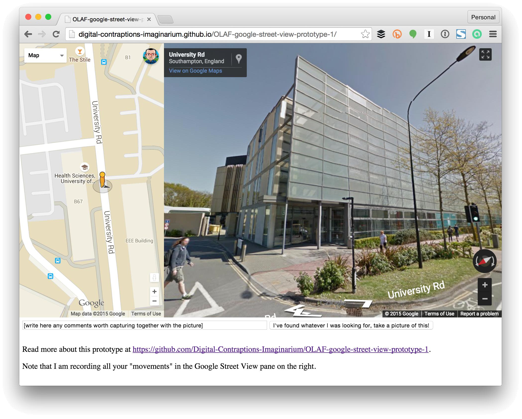
\includegraphics[width=0.95\textwidth]{some_picture.png}
	\caption{This picture should not be here, but apparently it is a nightmare in LaTeX.}
	\label{fig:some_figure}
\end{figure*}

\paragraph{}

Some text after.
	
\subsection{Scalability}

[THE CALL FOR PAPER EXPLICITLY SAYS THAT "EVIDENCE OF USE IN PRACTICE AND/OR DEMONSTRATION OF SCALABILITY IS REGARDED AS A PLUS"]

\subsection{{[}description of additional conditions to test X{]}}
\subsection{{[}description of additional conditions to test Y{]}}

\section{Experiment design}

\subsection{Research hypothesis}
\subsection{Dataset}
\subsection{Evaluation metrics}
\subsection{Experimental conditions}

\section{Results}

\section{Literature review}

\section{Discussion and conclusion}

\section*{Acknowledgments}

{[}The standard EPSRC acknowledgement formula + something about the external reviewers?{]}

\documentclass{article}
\usepackage{url}
\begin{document}
\nocite{*}
\bibliography{main}
\bibliographystyle{splncs03}
\end{document}


\end{document}

